\documentclass{beamer}
\title{Asal karim khorasani 970043474}
\author{Introduction to Automata Theory, Formal Languages and Computation}
\date{}
\usepackage{xcolor}
\usepackage{tikz}
\usetheme{warsaw}
\usecolortheme[named=purple]{structure}
\usebackgroundtemplate{
	
\includegraphics[width=\paperwidth , height=\paperheight]{me.jpg}
}


\begin{document}
\begin{frame}
		\maketitle
\end{frame}	
\begin{frame}
	\begin{center}
	\begin{tabular}{ccc}
		\hline
		& \multicolumn{2}{c}{Next State}\\
		\cline{2-3}
		\textbf{Present State } & \textbf{Z = 0} & \textbf{Z = 1}\\
		\hline
		A & (AB) &\\
		B & (CD) &\\
		C & & (CD)\\
		D & & (AB)\\
		(AB) & (AC)(AD)\\
		& (BC)(BD)\\
		(CD) & & (AC)(AD)\\
		& & (BC)(BD)\\
		(AC)\\
		(AD)\\
		(BC)\\
		(BD)\\
		\hline
		
	\end{tabular}
\end{center}

The testing table does not contain any repeated entry. The machine is an information lossless machine.


To fi nd the order of losslessness, a testing graph needs to be constructed.



\end{frame}	
\begin{frame}
	To fi nd the order of losslessness, a testing graph needs to be constructed.
	\begin{center}
		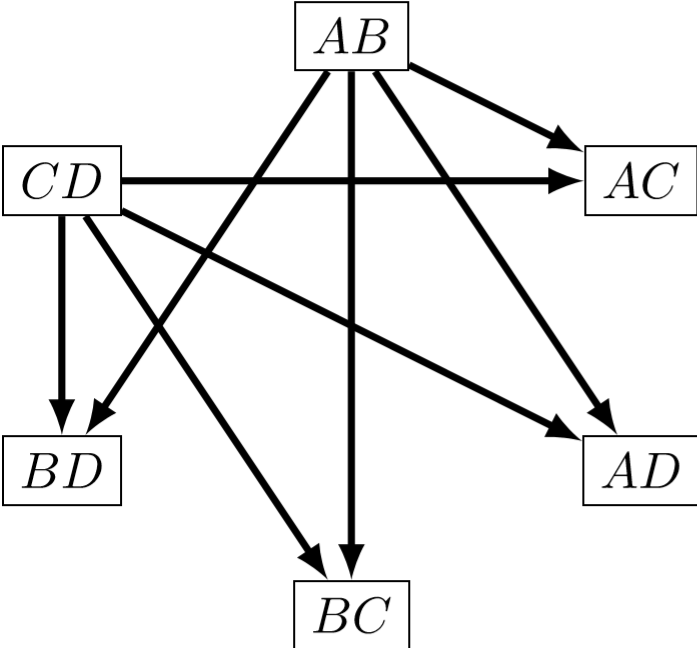
\includegraphics[height=120]{Screenshot .jpg}
	\end{center}
\end{frame}

\begin{frame}
	 The testing graph does not contain any loop. The order of losslessness is
	
	$\mu$ = 1 + 2 = 3. The length of the longest path of the graph is 1. 
	
	21. Find the input string which is applied on state ‘C’ producing the output string 1110000010 and the final state ‘B’ for the following machine.
	
\end{frame}	

\begin{frame}
	 \begin{center}
		\begin{tabular}{ccc}
			\hline
			&\multicolumn{2}{c}{Next State}\\
			\cline{2-3}
			\textbf{Present State} & \textbf{X = 0} & \textbf{X = 1}\\
			\hline
			A & E,1 & F,0\\
			B & D,0 & C,1\\
			C & F,1 & A,0\\
			D & C,0 & E,0\\
			E & B,0 & D,1\\
			F & D,1 & F,1\\
			\hline
		\end{tabular}
	\end{center}
\end{frame}	
\begin{frame}
	\textbf{Solution:} First, we need to prove that the machine is information lossless. For this, we need to construct a testing table for information lossless. If the machine is information lossless, then only a single input string can be found for a single beginning state and single fi nal state. The testing table for information lossless is
\end{frame}
\begin{frame}
	\begin{center}
		\begin{tabular}{ccc}
			\hline
			& \multicolumn{2}{c}{Next State}\\
			\cline{2-3}
			\textbf{Present State} & \textbf{Z = 0} & \textbf{Z = 1}\\
			\hline
			A & F & E\\
			B & D & C\\
			C & A & F\\
			D & (CE)\\
			E & B & D\\
			F & & (DF)\\
			\hline
			CE & AB & DF\\
			AB & DF & CE\\
			DF\\
			\hline
			
		\end{tabular}
	\end{center}
\end{frame}
\begin{frame}
	The testing table does not contain any repeated entry. The machine is an information lossless machine.
	
	The output successor table for the given machine is
	
	\begin{center}
		\begin{tabular}{ccc}
			\hline
			& \multicolumn{2}{c}{Next State , I/P}\\
			\cline{2-3}
			\textbf{Present State} & \textbf{Z = 0} & \textbf{Z = 1}\\
			\hline
			A & F,1 & E,0\\
			B & D,0 & C,1\\
			C & A,1 & F,0\\
			D & (C,0)\\
			& (E,1)\\
			E & B,0 & D,1\\
			F & & (D,0)\\
			& & (F,1)\\
			\hline
		\end{tabular}
	\end{center}
\end{frame}
	\begin{frame}
		The input string is applied on state C and has produced output 1. From the output successor table, it is clear that the next states are F with input 0. By this process, the transition is like the following
		
		
		The beginning state C and the fi nal state B are obtained from one path with the input string 0101000110. 
		
		22. Find the input string which is applied on state ‘D’ producing the output string 10011110 and the fi nal state ‘D’ for the following machine.
		
	\end{frame}
\begin{frame}
	\begin{center}
		\begin{tabular}{ccc}
			\hline
			& \multicolumn{2}{c}{Next State , Z}\\
			\cline{2-3}
			\textbf{Present State} & \textbf{X = 0} & \textbf{X = 1}\\
			\hline
			A & A,1 & C,1\\
			B & E,0 & B,1\\
			C & D,0 & A,0\\
			D & C,0 & B,0\\
			E & B,1 & A,0\\
			\hline
		\end{tabular}
	\end{center}
\textbf{Solution:} First, we need to prove that the machine is information lossless. For this, we need to construct a testing table for information lossless. If the machine is information lossless, then only a single input string can be found for a single beginning state and single fi nal state. The testing table for information lossless is
\end{frame}
\begin{frame}
	\begin{center}
		\begin{tabular}{ccc}
			\hline
			& \multicolumn{2}{c}{Next State}\\
			\cline{2-3}
			\textbf{Present State} & \textbf{Z = 0} & \textbf{Z = 1}\\
			\hline
			A & & (AC)\\
			B & E & B\\
			C & (AD)\\
			D &(BC)\\
			E & A & B\\
			\hline
			AC\\
			AD\\
			BC & (AE)(DE)\\
			AE & & (AB)(BC)\\
			DE & (AB)(AC)\\
			AB & & (AB)(BC)\\
			\hline
		\end{tabular}
	\end{center}
	
	The testing table does not contain any repeated entry. The machine is an information lossless machine. The output successor table for the given machine is
	
\end{frame}

\begin{frame}
	\begin{center}
		\begin{tabular}{ccc}
			\hline
			& \multicolumn{2}{c}{Next State , I/P}\\
			\cline{2-3}
			\textbf{Present State} & \textbf{Z = 0} & \textbf{Z = 1}\\
			\hline
			A & & (A,0),(C,1)\\
			B & E,0 & B,1\\
			C & (D,0),(A,1)\\
			D & (C,0),(B,1)\\
			E & A,1 & B,0\\
			\hline
		\end{tabular}
	\end{center}
	
	The transition is like the following
	
	The beginning state B and the fi nal state D are obtained from one path with the input string 10100010.
	
	23. Retrieve the input sequence from the machine when it was initially in state B, has, in response to yet unknown input sequence, produced the output sequence 01110, and terminated in state B.
\end{frame}

\begin{frame}
	\begin{center}
		\begin{tabular}{ccc}
			\hline
			& \multicolumn{2}{c}{Next State}\\
			\cline{2-3}
			\textbf{Present State} & \textbf{X = 0} & \textbf{X = 1}\\
			\hline
			A & A,0 & B,0\\
			B & C,0 & D,0\\
			C & D,1 & C,1\\
			D & B,1 & A,1\\
			\hline
		\end{tabular}
	\end{center} 
\end{frame}
\end{document}